\subsection{Parser}
The parser \ref{sec:parser} is the next step in the Action Interpreter, the objective is to create an AST \ref{sec:asttheory}, from the stream of tokens recieved by the scanner \ref{sec:ai_scanner}.\\
The AST returned by the parser is really simple, since only one command is analyzed at the time. The AST created from the tokens recieved by the scanner \ref{sec:ai_scanner} will look like \ref{pic:ai_parser_ast}.

\begin{figure}[H]
\begin{center}
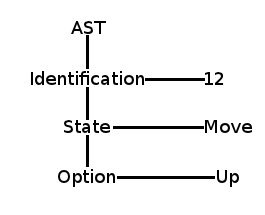
\includegraphics[scale=0.5]{Images/actioninterpreter/AST.png}
\end{center}
\caption{The AST parse from the stream of tokens recieved by the scanner.}
\label{pic:ai_parser_ast}
\end{figure}